\section{Evaluation}
\label{sec:aintea:validation}

We validated our approach by implementing a language named \langName{}, which features an uncertainty-aware static type system and provides the concepts and operators presented in \Cref{sec:aintea:duc}.
We evaluate the following two research questions based on our implementation of \langName{}:
\begin{itemize}
	\vspace{-0.5em}
	\setlength\itemsep{-0.3em}
	\item \textbf{RQ1:} Does native uncertainty management on the language level have an impact on the conciseness of a language, \ie its ability to express concisely statements? 
	\item \textbf{RQ2:} Can the type system detect errors related to uncertainty management?
\end{itemize}

To address them, we compared our implementation to two state-of-the-art frameworks: Infer.NET~\cite{url:InferNET18} and OpenTURNS~\cite{baudin2017openturns}.
The code used for the experiments of the validation is available on the repository of our implementation.
%The source code of our \langName{} implementation\footnote{\url{https://github.com/lmouline/aintea}} together with the experiments of the presented validation.%\footnote{\url{https://github.com/lmouline/aintea/tree/master/evaluation/2019-06-Journal}} are accessible on GitHub.

In this section, we first detail the implementation of the \langName{} language.
Then, we show that our solution can detect type errors earlier than the two solutions we compare our work to.
Before discussing the results, we compare the number of lines of codes required for the different solutions to perform uncertainty propagation.

\subsection[Ain'tea: our implementation]{\langName{}: our implementation}
%\label{sec:uminijava}

We use the Xtext language workbench\footnote{\url{http://www.eclipse.org/Xtext/}} to define the concrete syntax and the type checker of our language (static semantics).
Based on the concrete syntax, Xtext generates the abstract one.
We implement the dynamic semantics with K3\footnote{\url{http://diverse-project.github.io/k3/}}. 

In addition, we implemented different code samples which shows the different features of our language.%\footnote{\url{https://github.com/lmouline/aintea/tree/master/sample/tutorial/basics}}.
We also developed a simplified version of our use case example, introduced in \Cref{chapt:example}.
We presented it as a tutorial of our language.%\footnote{\url{https://lmouline.github.io/aintea/tutorial/creos-use-case/}}.
All code can be executed using a runner, available on the project repository.%\footnote{\url{https://github.com/lmouline/aintea/tree/master/duc.uscript.parent/duc.uscript.runner.standalone}}.

\subsubsection{Overview of the language}
\langName{} supports classes, with fields and functions.
It has an expression language with arithmetic and boolean expressions, \textit{IF-}conditions and affectation statements.

\langName{} is composed of four elements: an abstract syntax, a concrete syntax, static and dynamic semantics.
As depicted in Figure~\ref{fig:global-lang-arch}, the concrete syntax has been implemented using Xtext.
As we used a grammar-first approach, the abstract syntax has been automatically generated from the concrete one.
In addition, stub-classes are generated for the semantics (static and dynamic).
Using Xtend, we implement the static semantics.  
The dynamic semantics is defined as an operational semantics and implemented using K3~\cite{DBLP:journals/sosym/JezequelCBMF15}. 
The implementation of our uncertainty-aware type checker and semantic uses two strategies.
For simple operations (\textit{e.g.} operator semantics for uncertain booleans), we implement them using K3.
For more complex operations, like the computation of integral or combining different distributions, we use a third party library: Apache Commons Math Library\footnote{\url{http://commons.apache.org/proper/commons-math/}}.

Finally, by using the Xtext language workbench, other important features have been generated for our language.
Among them, there is the error maker, auto-completion and an Eclipse plugin.

\begin{figure}
	\centering
	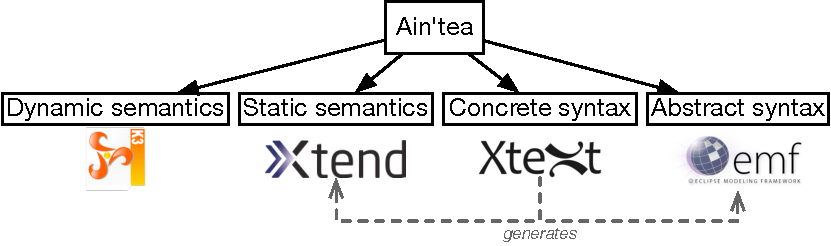
\includegraphics[width=0.8\linewidth]{img/chapt-aintea/impl/global2}
	\caption{Global architecture of Ain'tea}
	\label{fig:global-lang-arch}
\end{figure}

\subsubsection{Syntax}
The syntax of the language has been inspired by Java: keywords to define classes, fields and functions are similar. 
Regarding the uncertain operators defined in \Cref{sec:aintea:duc}, we use the same syntax as for certain operators where ever possible.
We give an overview of their corresponding syntax in the following list:
\begin{itemize}
    \item confidence: \textbf{[ ]}
    \item existence: \textbf{exist}
    \item cast: \textbf{as}
    \item dot: \textbf{.}
    \item inequality: \textbf{$>$}, \textbf{$>=$}, \textbf{$<$}, \textbf{$<=$}
    \item (uncertain) equality: \textbf{==}, \textbf{!=}
    \item identity: \textbf{===}, \textbf{!==}
    \item uncertain arithmetic: \textbf{+}, \textbf{-}, \textbf{*}, \textbf{/}
    \item uncertain boolean: \textbf{\&\&}, \textbf{$\|$}, \textbf{!} 
\end{itemize}

Inequality, arithmetic and boolean operators have identical syntax for uncertain and certain data.
By making this choice, combining uncertain or certain data is done with the same syntax.
For example, adding two uncertain numbers is performed by the following syntax: $u_{N1} + u_{N2}$.

When the equality operator (==, !=) is used with at least one uncertain data type, we apply the uncertain equality operator.
For example, the following code $u_{N1} == u_{N2}$ returns the confidence that both values are equal.
To use the identity operator, we use the following syntax: === and !==.
For example, this code $u_{N1} === u_{N2}$ checks if both uncertain numbers are identical (cf. Operator~\ref{op:s-equality}).

Following his name, the syntax of the dot operator is a dot (.).
The value can be accessed using the \textit{value} keyword.
For example, to get the value of an uncertain boolean, one will write $u_b.value$.
To get the probability distribution, the \textit{confidence} keyword has been introduced.
For example, the Bernoulli distribution of an uncertain boolean is resolved using the following syntax: $u_b.confidence$.

For the cast operator, we add the \textit{as} keyword.
For instance, to cast an uncertain number to a certain one, one will do $u_n\ as\ Number$.
Here, \textit{Number} represents any number type of our language: short, integer, long, float and double.

An internal method is used to call the existence operator: \textit{exist}.
For example, in order to check if a value of an uncertain boolean exists with at least 0.8 confidence, one needs to add the following line in its code: exist($u_B$, 0.8).

Finally, the confidence operator is called using square brackets: [ ].
For example, to get the most confidence value of an uncertain number with at least 0.7 as confidence, one will write: $u_N[0.7]$

\bigskip
The type of uncertain data can be thought of as a pair of two types: one for the raw data and one for the uncertainty representation.
We decide to use a syntax similar to the one used in Java to declare generic types: Type1$<$Type2$>$.
We arbitrarily choose to put the probability distribution for the first type and the type of the raw data point for the second.
For example, the declaration of an uncertain boolean is done using the following syntax: Bernoulli$<$bool$>$.

\subsubsection{Dependency and joint detection}
As we explained in~\Cref{sec:aintea:duc}, dependency and joint between two variables impact the semantics of the different operators.
In our implementation, we first consider that any variable initialized by a constant is independent.
Then, we compute a dependency graph between the different variables.
However, we use an algorithm which covers only the simple cases.

Concerning the joint, we also apply a simple and naive algorithm to compute the domain covered by boolean variables.
But, this is only performed on boolean resulting from comparison operators with one static constant.
We let for future work the implementation of an algorithm that applies the same rules at runtime.
Below, an example of what our implementation can do.

Let us imagine three uncertain booleans $b_1$, $b_2$, and $b_3$ defined as follow, with $u_n$ an uncertain number: 
\begin{itemize}
	\item $b_1 := u_n >= 10$
	\item $b_2 := u_n < 15$
	\item $b_3 := u_n > 20$
\end{itemize}

From this definition, $b_1$ is defined on the range $[10, +\infty)$, $b_2$ on $(-\infty, 15)$, and $b_3$ on $(20, +\infty)$.
$b_1$ and $b_2$ are thus non-disjoint, like $b_1$ and $b_3$.
Indeed, $b_1$ and $b_2$ are both defined on the range $[10, 15)$, and $b_1$ and $b_3$ on $(20, +\infty)$.
However, $b_2$ and $b_3$ are disjoint as it does not exist any common range between their definition.

\subsection{Conciseness}
Regarding the syntax, we distinguish three kinds of operations which manipulate data: writing\footnote{This operation also includes the creation and the deletion. 
The first one corresponds to the first write operation and the last one is done by setting the value to \textit{NULL}.}, reading, and combination. 
For these three kinds of operations, we compare the number of lines of codes required by our language and the two frameworks.
To perform this, we implemented a simplified version of our case study using these three solutions.
Excerpts of the source code are shown in Listing~\ref{lst:valid-expr-csharp}-\ref{lst:valid-expruscript}.

Writing and reading operations remain similar to what exists in many other programming languages.
There is no difference between the three solutions to this aspect.
In the listings, we can notice that all lines of code relative to it have the same size: line 6, 11, and 20 in Listing~\ref{lst:valid-expr-csharp}; line 7, 11-12, and 21 in Listing~\ref{lst:valid-expr-python}; and line 9, 16, and 27 in Listing~\ref{lst:valid-expruscript}.

Both languages used for developing the frameworks (C\#\footnote{\url{https://docs.microsoft.com/en-us/dotnet/csharp/programming-guide/statements-expressions-operators/overloadable-operators}} and Python\footnote{\url{https://docs.python.org/3/reference/datamodel.html\#special-method-names}}) allow overloading operators.
As highlighted in the listings, the three solutions have the same syntax to combine (through arithmetic or boolean operators) uncertain and certain data: lines 9 and 23 in Listing~\ref{lst:valid-expr-csharp}; lines 10 and 23 in Listing~\ref{lst:valid-expr-python}; and lines 13 and 34 in Listing~\ref{lst:valid-expruscript}.

In contrary to OpenTurns and our solution, Infer.NET requires an explicit call to the engine which computes and propagates the probabilities.
We can see these calls in line 10, 16 and 22 in Listing~\ref{lst:valid-expr-csharp}.
This framework is mainly done for probabilistic programming, where developers implement a model, then executes it.
From our understanding of this tool, it was not designed to allow an iterative propagation of uncertainty and a control flow that depends on this propagation.
Thus, we need to split the propagation in different models and explicitly call their inference engine to enable such a process.

Finally, all three solutions allow reasoning on uncertain data.
In Listing~\ref{lst:valid-expr-csharp} at line 17, Listing~\ref{lst:valid-expr-python} at line 18, and Listing~\ref{lst:valid-expruscript} at line 24, we highlight an IF-condition based on the confidence of an uncertain boolean\footnote{As OpenTurns does not include an uncertain boolean implementation, we implemented one similar to the one we provide in \langName{}, using their Bernoulli implementation. The implementation is  accessible in our GitHub repository}.
Infer.NET provides a method to help manipulate uncertain booleans, by providing methods to access the probability of the \true{} and \false{} value.
In this case, our confidence operator can be thought of as a sugar syntax of these methods.

\begin{lstlisting}[style=cSharpStyle, caption={Excerpt of the Infer.NET implementation (C\#)}, label=lst:valid-expr-csharp, linewidth=0.97\textwidth, escapechar=\%]
public void ComputeLoadNoCable(Substation substation) {
  Variable<bool> noCableConn = Variable.Bernoulli(1);
  if(substation.Fuses.Count > 0)
    noCableConn = substation.Fuses[0].IsClosed;
  else
    %\colorbox{highlightCode1}{substation.Load = GaussianFromMeanAndVariance(0, 0.001);}%
    return;
  for(int i=1; i<substation.Fuses.Count; i++)
    %\colorbox{highlightCode1}{noCableConn = noCableConn \& substation.Fuses[i].IsClosed;}%
  %\colorbox{highlightCode1}{Bernoulli bernoulli = (Bernoulli) InferenceEngine.Infer(noCableConn);}%
  %\colorbox{highlightCode1}{substation.Load = GaussianFromMeanAndVariance(0, bernoulli.GetVariance());}%
}

public void ComputeLoad(Substation substation) {
  Variable<bool> isDisco = substation.IsDisconnected();
  %\colorbox{highlightCode1}{Bernoulli bern = (Bernoulli) InferenceEngine.Infer(isDisco);}%
  %\colorbox{highlightCode1}{\textcolor{blue}{if}(bern.GetProbTrue() >= 0.95)}%
    ComputeLoadNoCable(substation);
    return;
  %\colorbox{highlightCode1}{Variable<double> load = GaussianFromMeanAndVariance(0, 0.001);}%
  foreach(Fuse fuse in substation.Fuses)
    %\colorbox{highlightCode1}{Bernoulli isClosedBern = (Bernoulli) InferenceEngine.Infer(fuse.IsClosed);}%                         
    %\colorbox{highlightCode1}{load = load + (fuse.Cable.Load * isClosedBern.GetProbTrue());}%
  substation.Load = load;
}
\end{lstlisting}

\begin{lstlisting}[style=pythonStyle, caption={Excerpt of the OpenTurns implementation (Python)}, label=lst:valid-expr-python, linewidth=0.97\textwidth, escapechar=\%]
def compute_load_no_cable(substation):
  if not isinstance(substation, Substation):
      raise TypeError('Wrong type')
  if len(substation.fuses) > 0:
      no_cable_conn = substation.fuses[0].isClosed
  else:
      %\colorbox{highlightCode1}{substation.load = ot.Normal(0, 0.001)}%
      return
  for fuse in substation.fuses[1:]:
      %\colorbox{highlightCode1}{no\_cable\_conn = no\_cable\_conn \& fuse.isClosed}%
  %\colorbox{highlightCode1}{substation.load = ot.Normal(0,~~~~~~~~~~~~~~~~~~~~~~~~~~~~~~~~~~~~~~~~~~~~~}%
  %\colorbox{highlightCode1}{~~no\_cable\_conn.getStandardDeviation()*no\_cable\_conn.getStandardDeviation())}%

def compute_load(substation):
  if not isinstance(substation, Substation):
      raise TypeError('Wrong type')
  is_disco = substation.is_disconnected()
  %\colorbox{highlightCode1}{\textcolor{blue}{if} is\_disco.exist(0.95) and is\_disco.value\_with\_confidence(0.95):}%
      compute_load_no_cable(substation)
      return
  %\colorbox{highlightCode1}{load = ot.Normal(0, 0.001)}%
  for fuse in substation.fuses:
      %\colorbox{highlightCode1}{load = load + (fuse.cable.load*fuse.isClosed.confidence.getP())}%
  substation.load = load	
\end{lstlisting}

\begin{lstlisting}[style=uMiniJavaStyle, caption={Excerpt of the \langName{} implementation}, label=lst:valid-expruscript, linewidth=0.97\textwidth, escapechar=\%]
void ComputeLoadNoCable(Substation substation) {
  Bernoulli<bool> noCableConn = new Bernoulli<bool>(true, 1);
  Fuse[] fuses = substation.fuses;
  Fuse f;
  if(fuses.length > 0) 
    f = fuses[0];
    noCableConn = f.isClosed;
  else
    %\colorbox{highlightCode1}{substation.load = new Gaussian<double>(0, 0.001);}%
    return;
  for(int i=1; i<fuses.length; i=i+1)
    f = fuses[i];
    %\colorbox{highlightCode1}{noCableConn = noCableConn \&\& f.isClosed;}%
  Bernoulli bern = noCableConn.confidence;
  if(bern.probability >= 0.97) {
    %\colorbox{highlightCode1}{substation.load = new Gaussian<double>(0, 0.0289);}%
  } else {
    [...]
  }
}

void ComputeLoad(Substation substation) {
  Bernoulli<bool> isDisco = substation.isDisconnected();
  %\colorbox{highlightCode1}{\textcolor{blue}{if}(exist(isDisco, 0.95) \&\& isDisco[0.95])}%
    ComputeLoadNoCable(substation);
    return;
  %\colorbox{highlightCode1}{Gaussian<double> load = new Gaussian<double>(0, 0.001);}%
  Fuse[] fuses = substation.fuses;
  for(int i=0; i<fuses.length; i=i+1)
    Fuse f = fuses[i];
    Cable c = f.cable;
    Bernoulli<bool> isClosed = f.isClosed;
    Bernoulli bern = isClosed.confidence;
    %\colorbox{highlightCode1}{load = load + c.load * bern.probability;}%
  substation.load = load;
}
\end{lstlisting}


RQ1 aims at evaluating the impact of native uncertainty management on the conciseness of a language.
As shown by the above evaluation, adding uncertainty as a first-class citizen can be done without damaging the conciseness.
As we have seen through this paper, managing uncertainty impacts the semantics of the language, by complexifying the traditional operators (arithmetic, boolean, comparison).
A few operators can also be added in order to enable reasoning over the uncertainty.
The impact on the concrete syntax is thus limited.

However, developers will use the same syntax to manipulate more complex concepts.
Adding two uncertain numbers and two numbers is semantically different.
One threat to validity is the lack of impact assessment on developers, who may have difficulty manipulating these concepts.
However, as we hide this complexity behind traditional operators, the risk is rather low.


\subsection{Error handling at development time}
Among the different root causes of typing errors, one is code refactoring.
In order to validate our approach, we thus define a scenario based on it.

Let's assume a developer implements the load approximation for a smart grid.
% Ludo: I keep the last part of the comment for after the first review. I addressed the first part
%\tha{[...] Why not simply using one of the examples used in the other papers related to uncertainty? Or why not using something more mathematical?}
She/he must consider different scenarios that can exist from a simple cable to a more complex situation which looks like a small graph.
As the code is complex, in one place (\eg a file) she/he defines the smart grid classes and she/he implements this computation in another one.
At first, the developer decides to use the Dirac delta function to represent the uncertainty of the substation load.
During the development process, she/he notices that the Gaussian one suit more his/her problem.
However, all the operations are not compatible with this new type, for example when there is no cable connected.

As we depict in Figure~\ref{fig:valid-error-handling}, our approach can detect this type of error statically.
Plus, we can also notice that we can help developers fix this kind of issue by listing the compatible types with the new substation type (\textit{Gaussian$<$double$>$}).

\begin{figure}
    \centering
    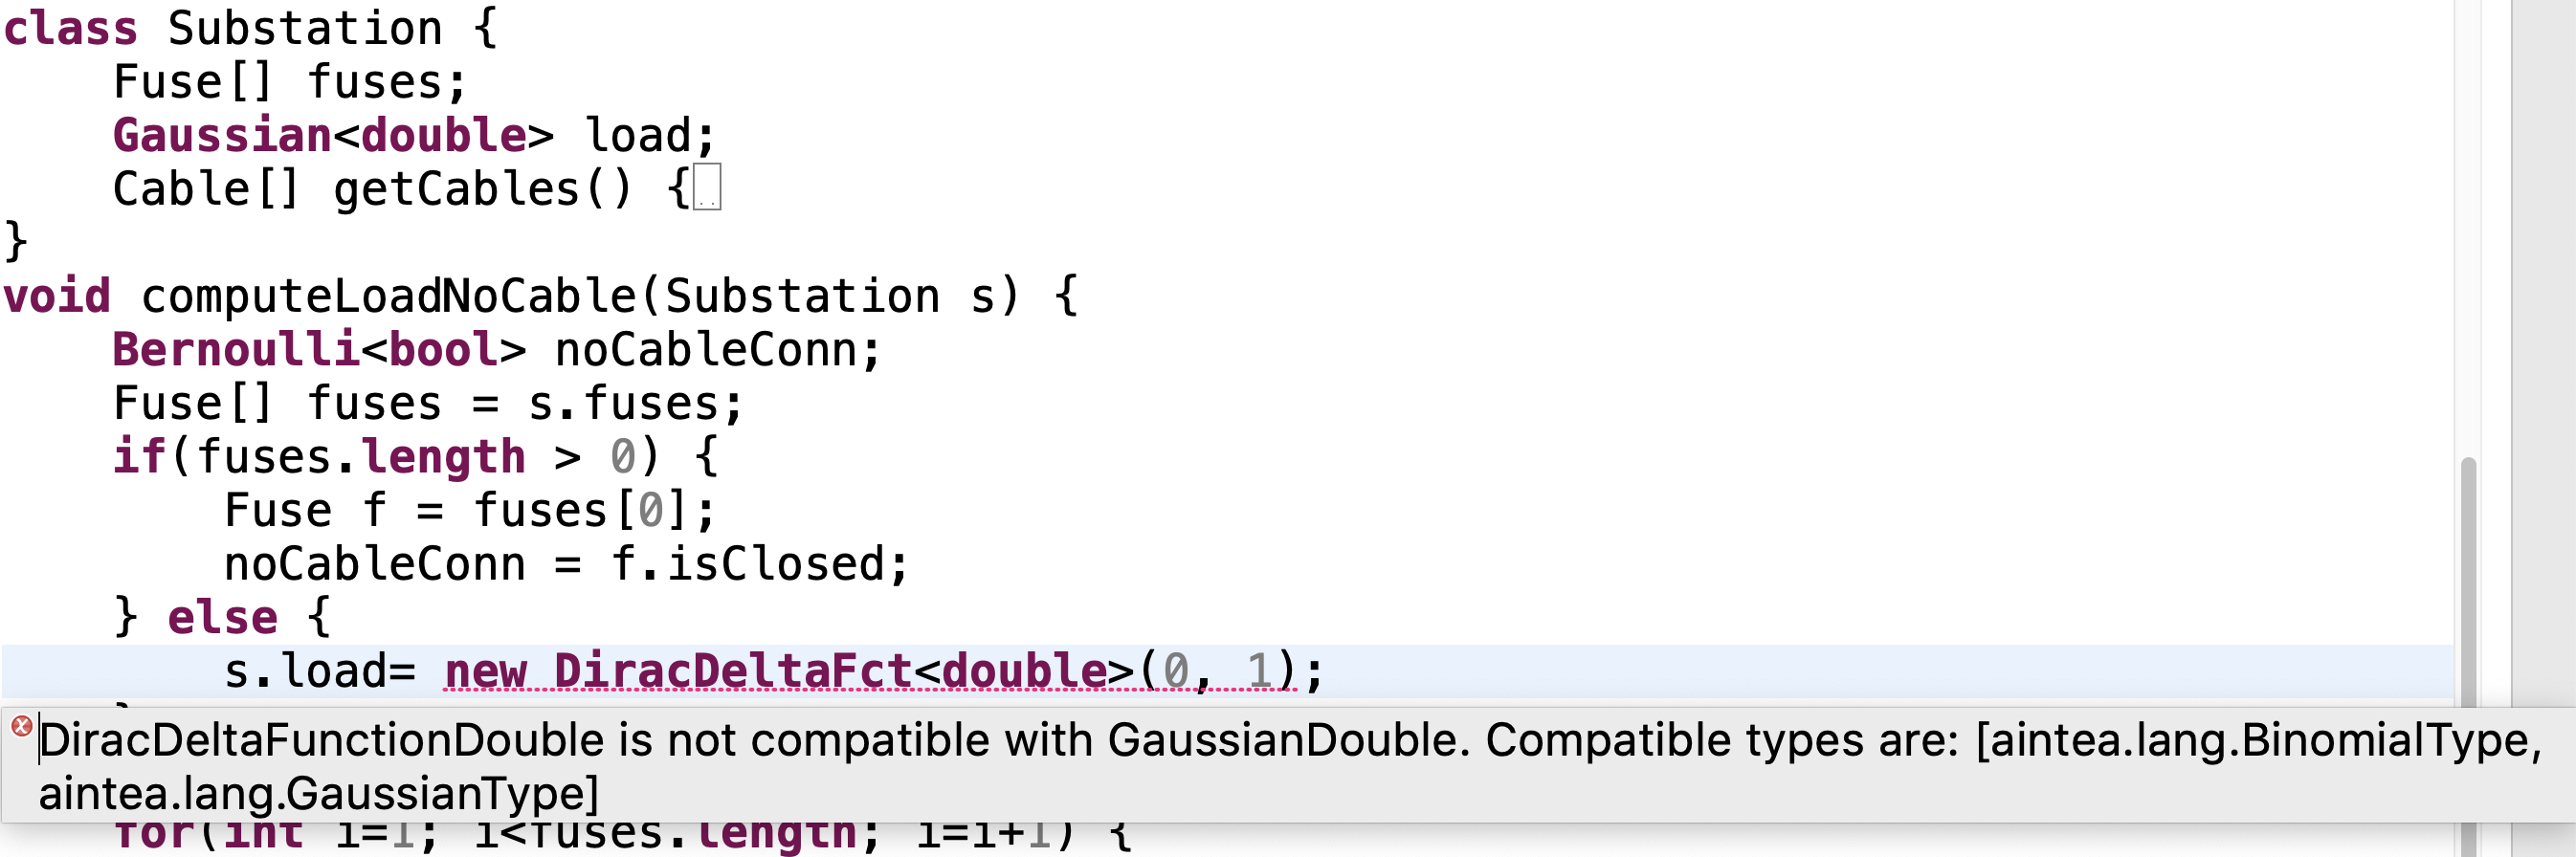
\includegraphics[width=0.9\linewidth]{img/chapt-aintea/valid/ErrorHandling-Refactoring}
    \caption{Detection of a type error}
    \label{fig:valid-error-handling}
\end{figure}

Among the two selected framework, only Infer.NET is implemented in a language which supports static type checking: C\#\footnote{\url{https://docs.microsoft.com/en-us/dotnet/csharp/programming-guide/types/index}}.
We also implement a simplified example that raises a typing error.
To do so, we perform an addition between two incompatible probability distributions: a Gaussian and a Gamma\footnote{The Rayleigh distribution is not present in the framework. We thus choose another one.}.
As we show in Figure~\ref{fig:valid-error-handling-csharp-global}, the error is only detected at runtime.

\begin{figure*}[ht]
	\centering
	\subfloat[Code with a type error, detected at the green highlighted line] {
		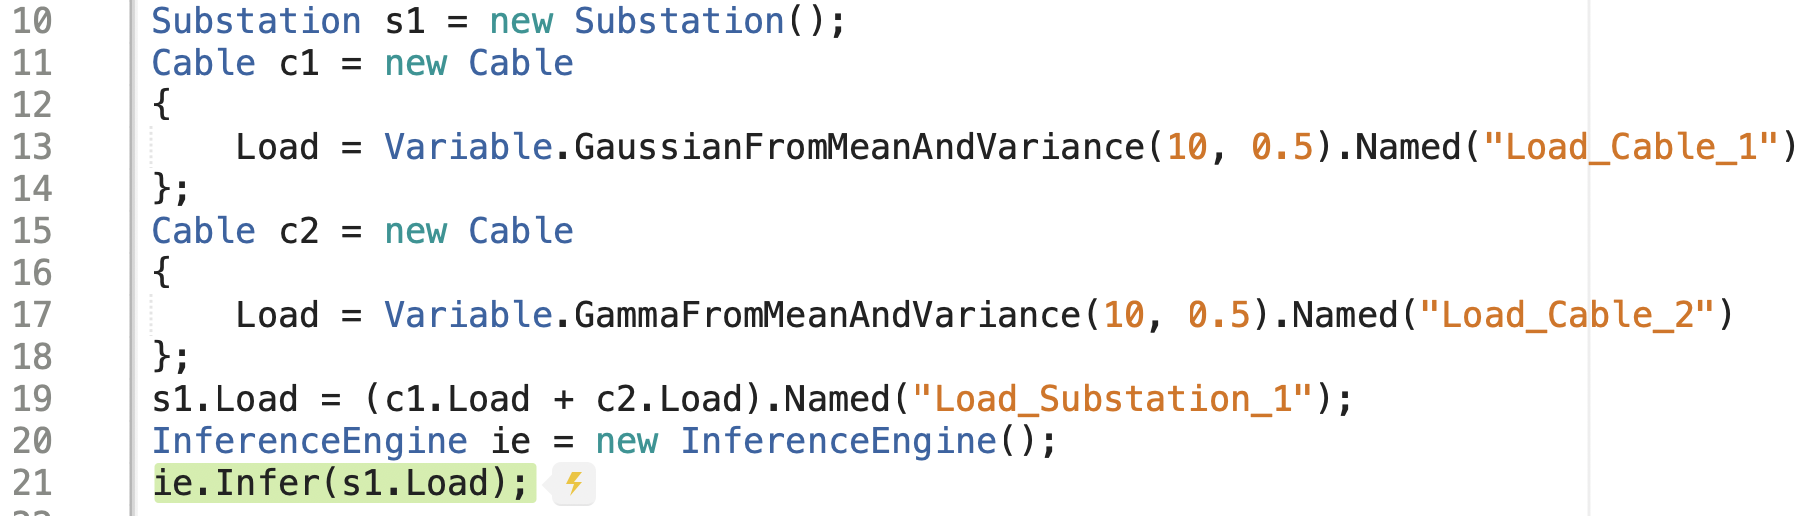
\includegraphics[width=.9\linewidth]{img/chapt-aintea/valid/ErrorHandling-CSharp-Code}
		\label{fig:valid-error-handling-csharp-code}
	}
	\hfill
    \subfloat[Console output] {
		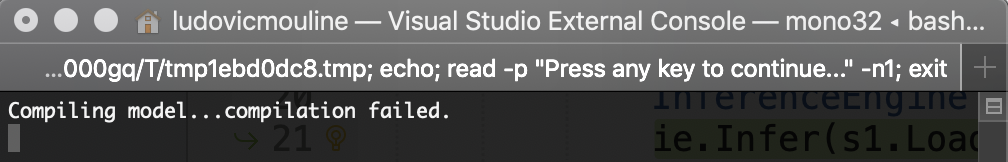
\includegraphics[width=.6\linewidth]{img/chapt-aintea/valid/ErrorHandling-CSharp-Terminal}
%		\label{fig:valid-error-handling-csharp-console}
	}
	\hfill
	\subfloat[Excerpt of the error message] {
		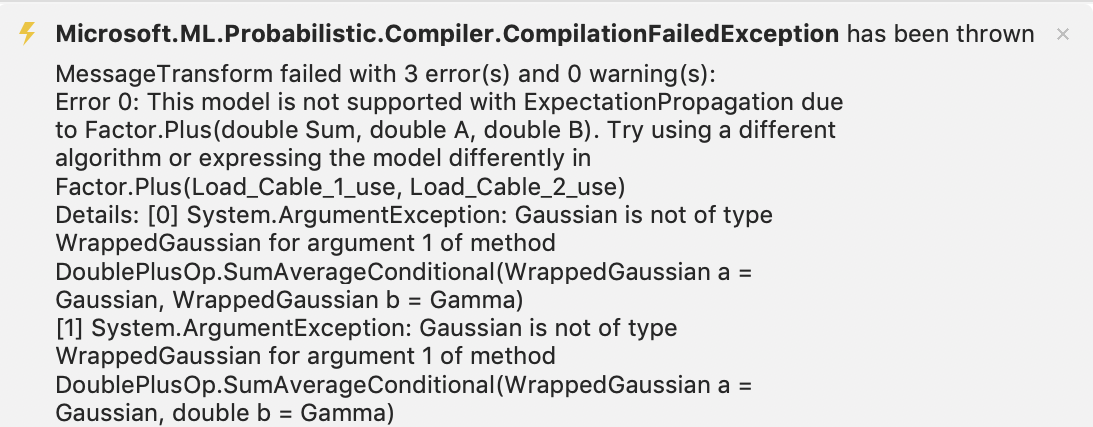
\includegraphics[width=.65\linewidth]{img/chapt-aintea/valid/ErrorHandling-CSharp-ErrorMsg-2}
%		\label{fig:valid-error-handling-csharp-error-msg}
	}
	\caption{Infer.NET detect the error at runtime.}
	\label{fig:valid-error-handling-csharp-global}
\end{figure*}

In addition, we see in Figure~\ref{fig:valid-error-handling} that by specifying the type system, the language is able to provide high-level explanations of the errors.
Here, it explains that the two distributions are not compatible plus gives the list of compatible distributions with the field type.
In contrary, in Figure~\ref{fig:valid-error-handling-csharp-global}, the error is detected later than its root cause and informs that the operation is not supported.
Indeed, as depicted in Figure~\ref{fig:valid-error-handling-csharp-code}, the error of line 19 is detected at line 21 (highlighted in green) without any reference to this operation.
Plus, the error message detailed all type mismatches between the declaration of the method and the given types.

This evaluation validates the ability of a type system to detect errors related to uncertainty management (RQ2).
When a type system is implemented, error messages are defined to help developers.
And so, support to develop uncertainty-aware software can be provided. 

\subsection{Discussion}

By mapping arithmetic and boolean operators to the propagation of uncertainty, we hide the complexity of the combination of probability distributions.
It helps developers to stay in the paradigm that they use every day, introducing as few concepts as possible.
This being said, as we intend to have a language that manipulates several kinds of uncertainties, they still need a high-level knowledge of probability distributions.
For example, they should understand the difference between a Gaussian and a Rayleigh.
But they do not need to know if or how they can be combined.
Indeed, thanks to our type checker, the language will provide information or raise errors when it is not possible.

However, if the uncertainty of a domain can be represented using only one probability distribution, thus this distribution could also be hidden for the developer.
Therefore, they will only manipulate uncertain and certain data.
For example, using the approach introduced in~\cite{DBLP:conf/sle/MayerhoferWV16}, a developer will only manipulate \textit{UReal} and \textit{Real} for uncertain and certain numbers.

By hiding the complexity of the combination of probability distributions, we also hide the computation overhead introduced.
This work has not been done with performance as a goal.
We do not guarantee any performance of our language.
The evaluation lacks a quantification of this overhead.